\documentclass[tikz,border=10pt]{standalone}
\usetikzlibrary{arrows.meta, positioning, shapes.geometric}

\begin{document}
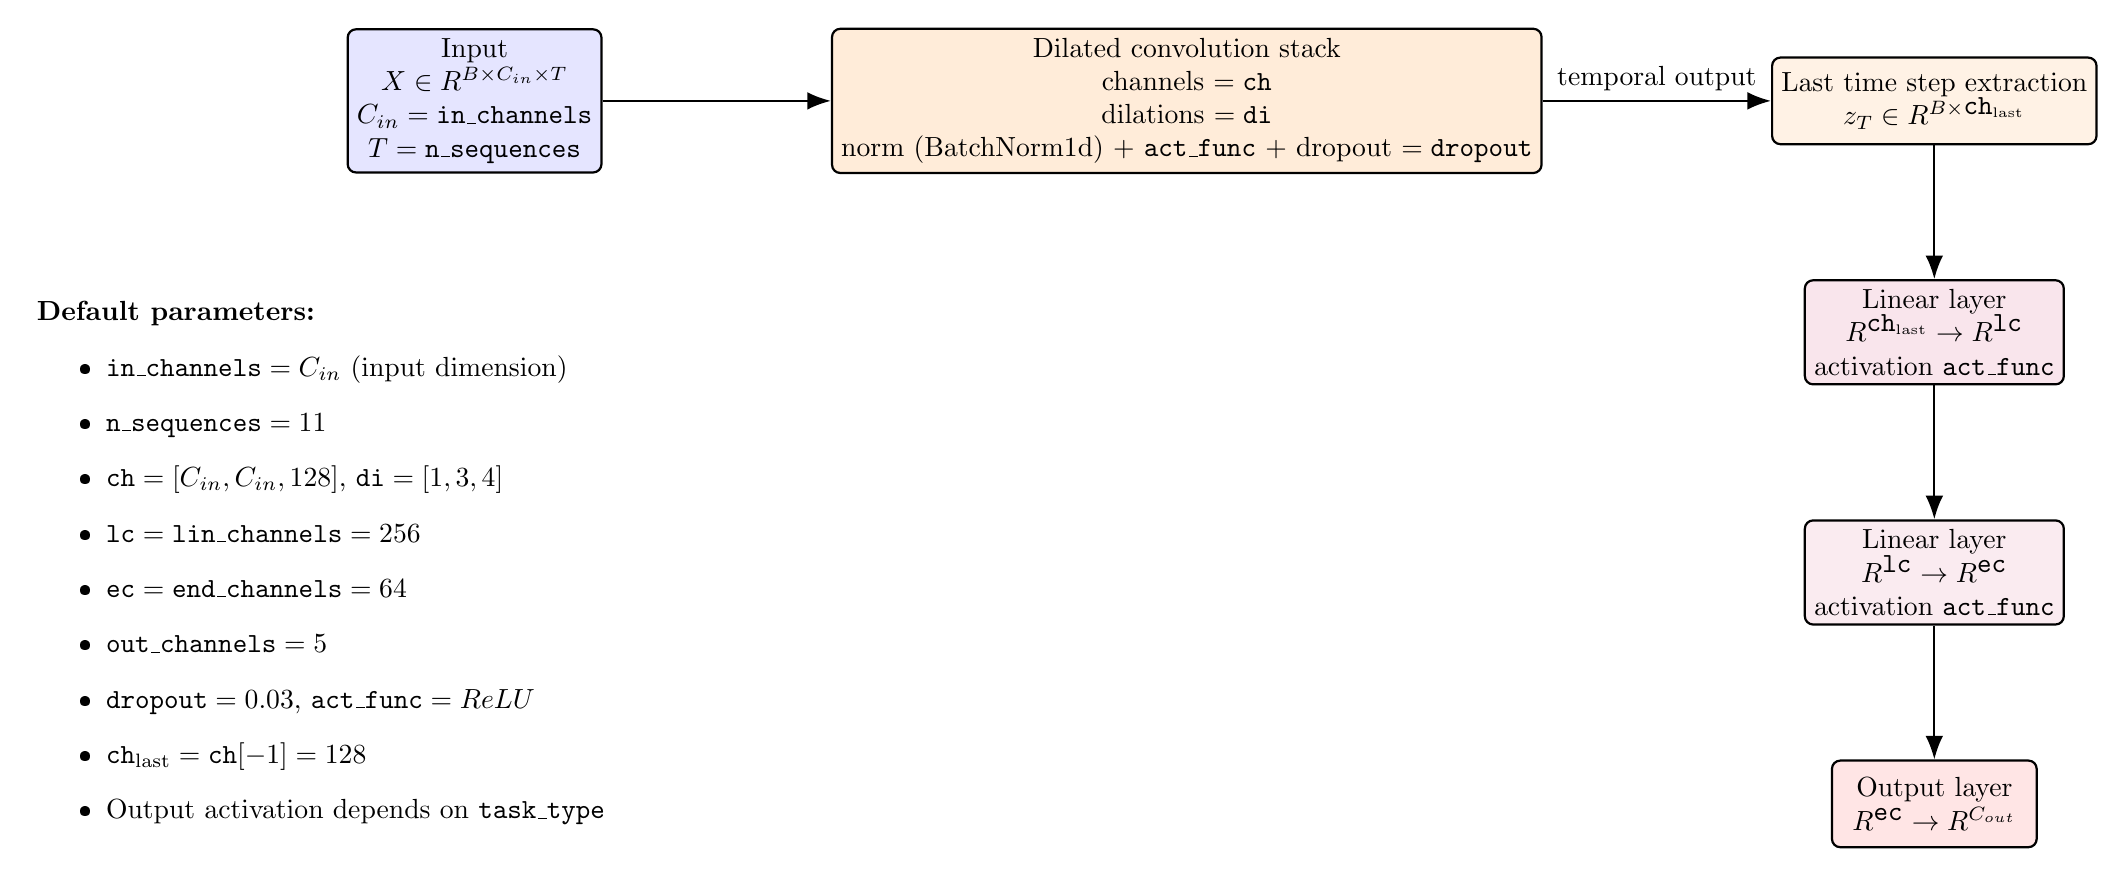
\begin{tikzpicture}[
    block/.style={draw, thick, minimum width=2.6cm, minimum height=1.1cm, align=center, rounded corners=3pt},
    arrow/.style={-{Latex[length=3mm]}, thick}
]
    % Input sequence information
    \node[block, fill=blue!10] (input) {Input\\$X \in \mathbb{R}^{B \times C_{in} \times T}$\\
        $C_{in} = \texttt{in\_channels}$\\
        $T = \texttt{n\_sequences}$};

    % Dilated convolution stack
    \node[block, right=2.9cm of input, fill=orange!15] (dilated) {Dilated convolution stack\\
        channels $= \texttt{ch}$\\
        dilations $= \texttt{di}$\\
        norm (BatchNorm1d) + $\texttt{act\_func}$ + dropout $= \texttt{dropout}$};

    \draw[arrow] (input) -- (dilated);

    % Last timestep extraction
    \node[block, right=2.9cm of dilated, fill=orange!10] (last) {Last time step extraction\\
        $z_T \in \mathbb{R}^{B \times \texttt{ch}_{\mathrm{last}}}$};

    \draw[arrow] (dilated) -- node[above]{temporal output} (last);

    % Linear layers and activations
    \node[block, below=1.7cm of last, fill=purple!10] (linear1) {Linear layer\\$\mathbb{R}^{\texttt{ch}_{\mathrm{last}}} \rightarrow \mathbb{R}^{\texttt{lc}}$\\
        activation $\texttt{act\_func}$};

    \draw[arrow] (last) -- (linear1);

    \node[block, below=1.7cm of linear1, fill=purple!8] (linear2) {Linear layer\\$\mathbb{R}^{\texttt{lc}} \rightarrow \mathbb{R}^{\texttt{ec}}$\\
        activation $\texttt{act\_func}$};

    \draw[arrow] (linear1) -- (linear2);

    \node[block, below=1.7cm of linear2, fill=red!10] (output) {Output layer\\$\mathbb{R}^{\texttt{ec}} \rightarrow \mathbb{R}^{C_{out}}$};

    \draw[arrow] (linear2) -- (output);

    % Legends for parameters
    \node[below=1.5cm of input, align=left] (legend) {
        \begin{minipage}{11cm}
            \textbf{Default parameters:}
            \begin{itemize}
                \item $\texttt{in\_channels} = C_{in}$ (input dimension)
                \item $\texttt{n\_sequences} = 11$
                \item $\texttt{ch} = [C_{in}, C_{in}, 128]$, $\texttt{di} = [1, 3, 4]$
                \item $\texttt{lc} = \texttt{lin\_channels} = 256$
                \item $\texttt{ec} = \texttt{end\_channels} = 64$
                \item $\texttt{out\_channels} = 5$
                \item $\texttt{dropout} = 0.03$, $\texttt{act\_func} = \text{ReLU}$
                \item $\texttt{ch}_{\mathrm{last}} = \texttt{ch}[-1] = 128$
                \item Output activation depends on $\texttt{task\_type}$
            \end{itemize}
        \end{minipage}
    };

\end{tikzpicture}
\end{document}
